\documentclass[UTF8]{article}
\usepackage{ctex}
\usepackage{amsmath}
\usepackage{graphicx}
\usepackage{listings}
\usepackage{xcolor}
\usepackage{geometry}
\usepackage{textcomp}
\usepackage{subfigure}
\geometry{left=4cm,right=4cm}
\definecolor{dkgreen}{rgb}{0,0.6,0}
\definecolor{gray}{rgb}{0.5,0.5,0.5}
\definecolor{mauve}{rgb}{0.58,0,0.82}

\lstset{ %
	language=java,                % the language of the code
	basicstyle=\footnotesize,   % 代码字体大小
	numbers=left,                   % where to put the line-numbers
	numberstyle=\tiny\color{gray},  % 行号颜色
	stepnumber=1,                   % 行行号隔几行标注一次
	numbersep=5pt,                  % how far the line-numbers are from the code
	backgroundcolor=\color{white},      % choose the background color. You must add \usepackage{color}
	showspaces=false,               % show spaces adding particular underscores
	showstringspaces=false,         % underline spaces within strings
	showtabs=false,                 % show tabs within strings adding particular underscores
	frame=single,                   % adds a frame around the code
	rulecolor=\color{black},        % if not set, the frame-color may be changed on line-breaks within not-black text (e.g. commens (green here))
	tabsize=2,                      % 行首和边框的距离
	captionpos=b,                   % sets the caption-position to bottom
	breaklines=true,                % sets automatic line breaking
	breakatwhitespace=false,        % sets if automatic breaks should only happen at whitespace
	title=\lstname,                   % show the filename of files included with \lstinputlisting;
	% also try caption instead of title
	keywordstyle=\color{blue},          % keyword style
	commentstyle=\color{dkgreen},       % comment style
	stringstyle=\color{mauve},         % string literal style
	escapeinside={\%*}{*)},            % if you want to add LaTeX within your code
	morekeywords={*,...}              % if you want to add more keywords to the set	
}

\begin{document}
\title{用搜索解决bait游戏}
\author{陈璐 181250012 chenlu@smail.nju.edu.cn}

\maketitle

\tableofcontents

\section{深度优先搜索}

\subsection{基本思想}
\indent 1、在游戏最开始时调用深度优先搜索函数获得一个可行的动作序列,之后在每次行动中依次输出动作。\\
\indent 2、深度优先搜索的基本过程为:从源结点开始,不断探索当前结点的下一个未探索结点,当所有此结点无子节点或所有子节点都被访问时进行回溯,直到找到目标结点或探索完所有结点。\\
\indent 3、在此游戏中,将每一个游戏状态(某一局面)作为点,将可行的行动作为边,构建图结构,并将初始状态作为源节点。

\subsection{实现方法}

\begin{lstlisting}[caption=深度优先搜索]
 private void depth_first(StateObservation stateObs){
		 if(stateObs.isGameOver()) game_over = true;
		 if(game_over) return;
		 
		 ArrayList<Types.ACTIONS> actions = stateObs.getAvailableActions();
		 /* not necessarily the optimal solution */
		 for(int i = 0; !game_over && i < actions.size(); i++){
				 StateObservation stCopy = stateObs.copy();
				 Types.ACTIONS one_action = actions.get(i);
				 stCopy.advance(one_action);
				 if(!reached(stCopy)) {
						 optimal_action.add(one_action);
						 reached_state.add(stCopy);
						 depth_first(stCopy);
				 }
		 }
		 
		 if(game_over == false){
				 if(optimal_action.size() != 0)
						optimal_action.remove(optimal_action.size()-1);
				 if(reached_state.size() != 0)
				 		reached_state.remove(reached_state.size()-1);
		 }
		 return;
 }
\end{lstlisting}

\noindent\textbf{主要实现过程}\\
\indent 如上所示,在整个过程中维护reached\_state和optimal\_action(或许叫这个名字不太合适)数组,分别表示初始状态到当前状态经过的所有状态序列和对应的行动,深度优先搜索的实现过程主要分为以下三步:\\
\indent 1、判断整个搜索过程是否结束(line 2-3):对于每一个状态,通过isGameOver函数判断游戏是否结束,当游戏结束时数组不再改变,依次返回退出递归过程,此时数组中储存的数据即为解序列。\\
\indent 2、探索所有子节点(line 5-16):假设初始状态为s,目标状态为G,在每一个循环中,都对当前状态a的所有次态B进行探索,若b($b\in B$)不在a的状态序列中,说明可能存在一条从s出发,经过a,b并到达g($g\in G$)的路,因此将b以及对应行动加入到数组中,并接着探索b,反之,假设b在a的状态序列中,说明此时s到a的路已经经过了b,那么再加入b到状态序列中就形成了环,此时将环去掉能够获得更好的解,因此无需探索b,从而对整个探索过程进行剪枝,降低复杂度。\\
\indent 3、回溯(line 18-23):再当前状态的所有次态均被探索时,如果游戏仍未结束,说明不存在经过次状态的解,或存在更好的解,因此将其移除,进行回溯。\\

\noindent\textbf{其他细节}\\
\indent 1、判断某个状态是否已经到达:调用提供的接口函数,将当前状态依次与数组中每个状态进行比较。
\begin{lstlisting}[caption=判断状态是否已经到达]
private boolean reached(StateObservation st){
		if(reached_state.size() == 0) return false;
		for(int i = 0; i < reached_state.size(); i++){
				if(st.equalPosition(reached_state.get(i))) return true;    
		}
		return false;
}
\end{lstlisting}

\indent 2、输出状态序列:设置指示变量AtBegin判断是否为第一次行动前,如果是则计算获得行动序列。否则说明行动序列已经得到,则通过变量cou输出行动序列。

\begin{lstlisting}[caption=输出行动序列]
public Types.ACTIONS act(StateObservation stateObs, ElapsedCpuTimer elapsedTimer){
		StateObservation newstateob = stateObs.copy();
		if(AtBegin) {
				cou = 0;
				reached_state.add(stateObs);
				depth_first(newstateob);
				AtBegin = false;
		}
		
		Types.ACTIONS action = null ;
		if(cou < optimal_action.size())
		action = optimal_action.get(cou);
		cou ++;
		return action;
}
\end{lstlisting}

\subsection{算法分析及改进}
\indent 此阶段使用的为一般的深度优先搜索,因此也具有一般深度优先搜索所具有的特点,如:算法搜索到的第一个解并不一定是最优解,(针对于第零关的环境,输出的解如图1所示)。\\
\indent 而为了获得全局最优解,可以将当前最优解序列存储起来,每次获得新解时进行更新,搜索完所有解空间后进行输出。并且为了使得解严格定义,且保证效率,可以采用深度受限的深度优先搜索进行实现,当搜索到解时不再加大深度,而是在搜索完毕后输出此时的最优解。\\

\begin{figure}[ht]
	\centering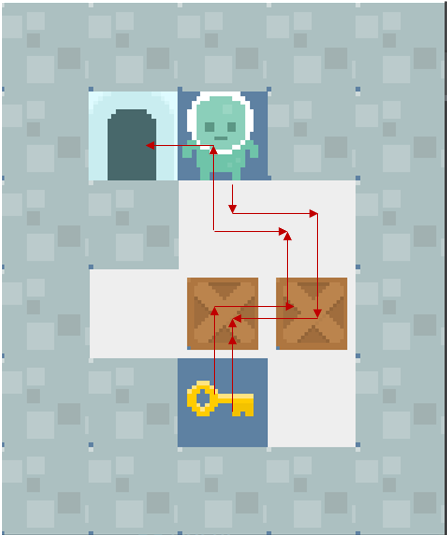
\includegraphics[width=7cm]{ai1-1.png}
	\caption{算法应用于第零关}
\end{figure}

\section{深度受限的深度优先搜索}

\subsection{基本思想}
\indent 基于节省单次运行时间考虑,采用深度受限的深度优先搜索,在每一个状态进行搜索,每次不必搜索到解,而是搜索到一定层数后,通过对状态好坏进行评估,从而对某次行动进行评估,并贪心执行最优的行动。\\

\begin{figure}[ht]
	\centering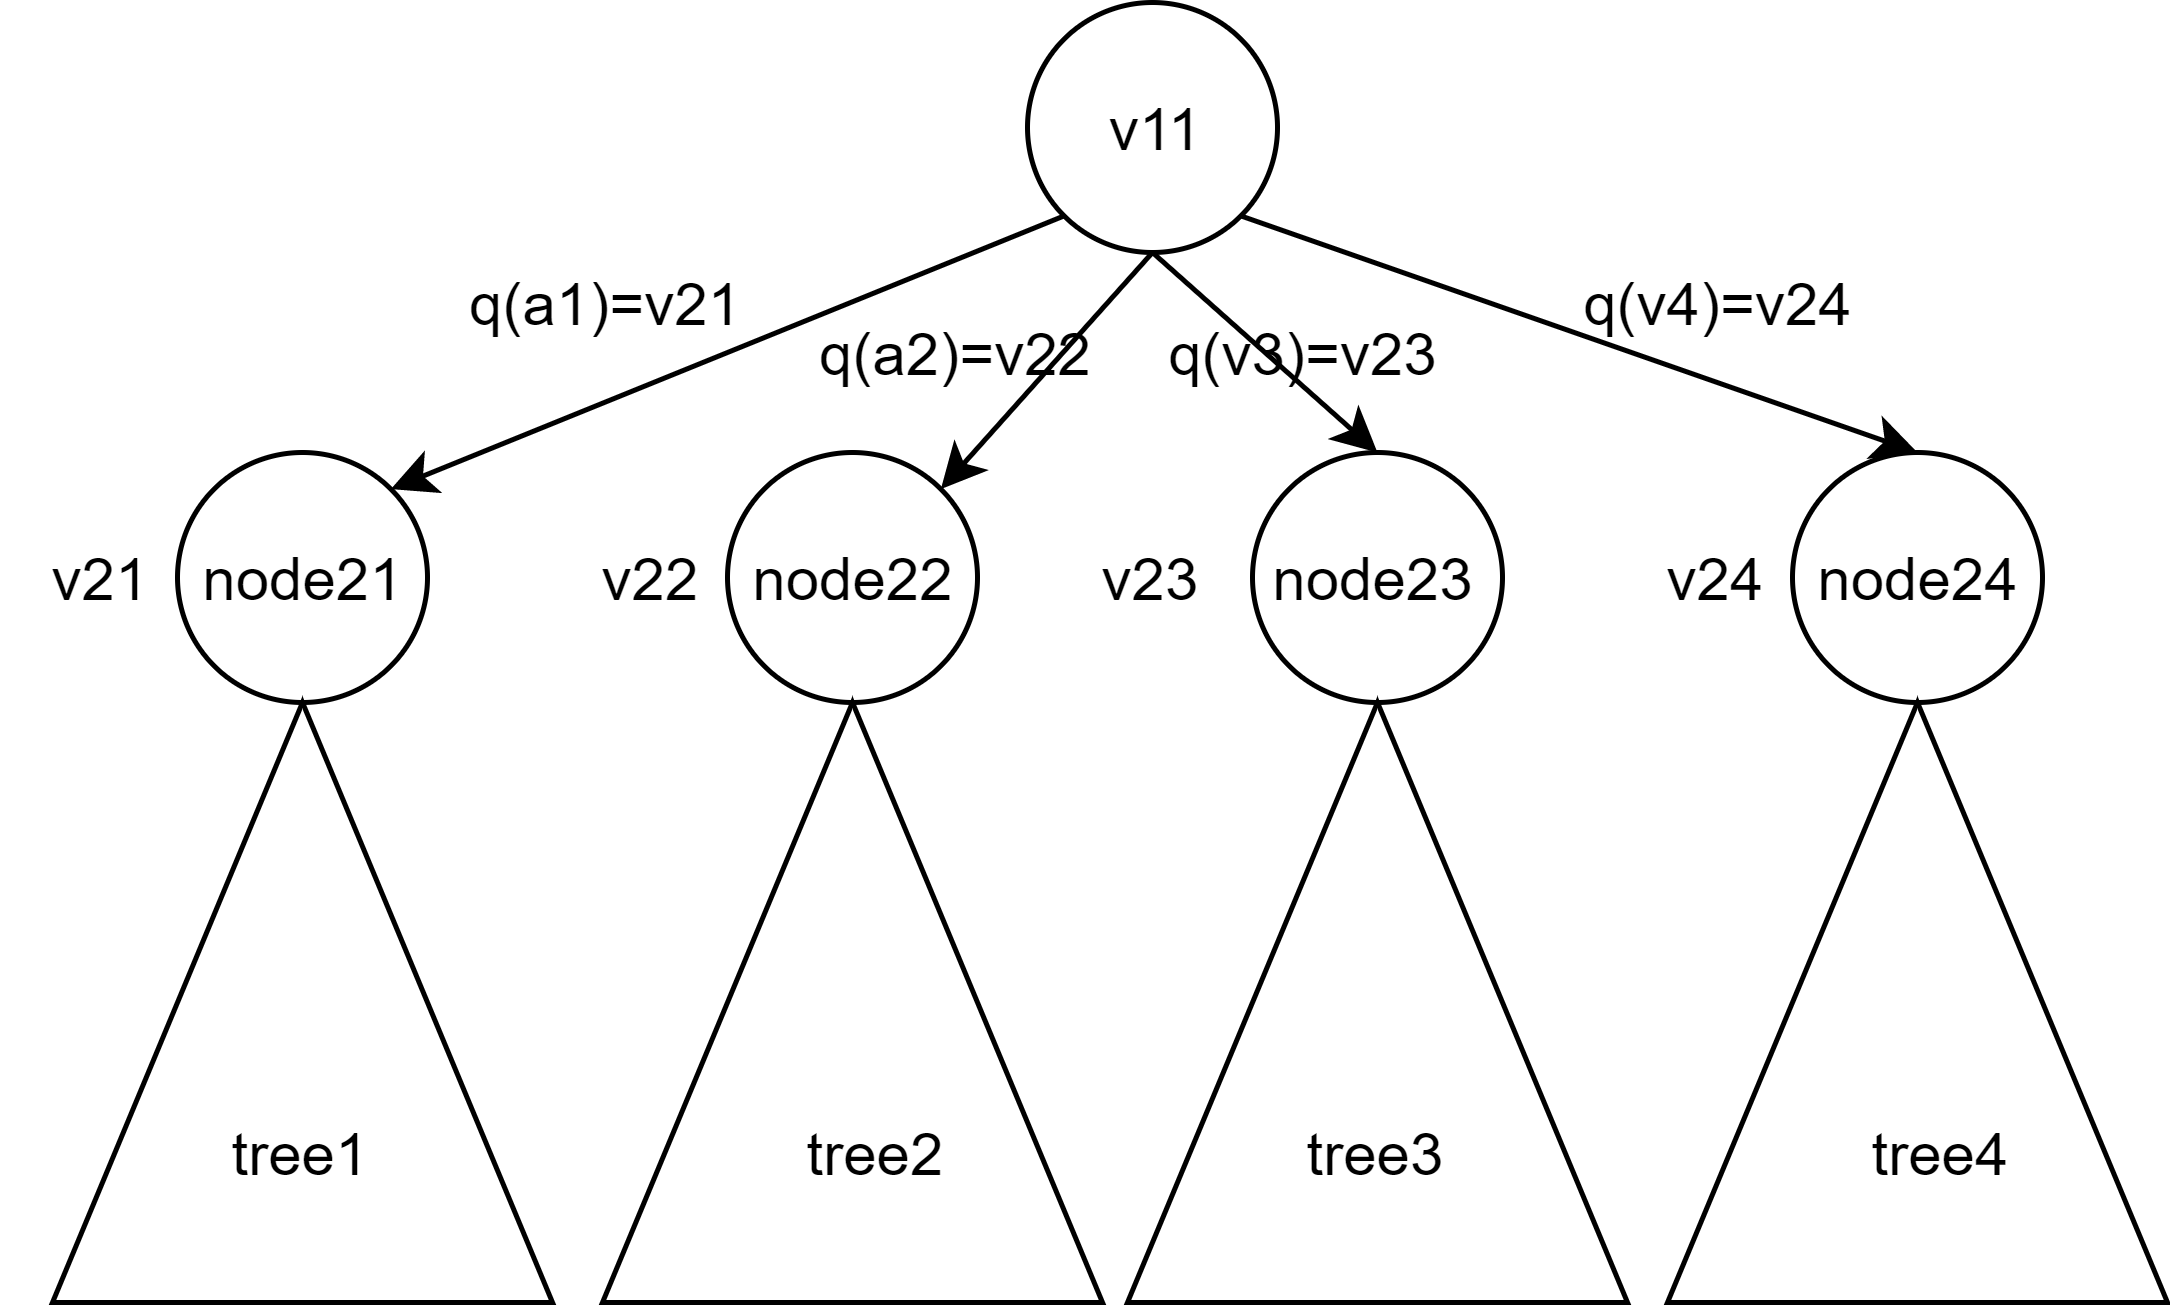
\includegraphics[width=10cm]{ai1-2.png}
	\caption{深度受限的深度优先搜索}
\end{figure}

\indent 如图2所示,某一个行动的权等于它所能到达的状态的权值,而每个非初始状态的权等于其所有行动的权和自身状态的评估w的最小值,以图中所示为例,有

\begin{equation}
\begin{cases}
v_{2i} = min(eval(v_{2i}),\ min_{action\ a\ of\ node_{2i}} q(a))\qquad& (1-1)\\
select\_action = argmin_i\ q(a_i)\qquad&(1-2)\\
\end{cases}	
\end{equation}

\subsection{算法实现}
\indent 应用2.1部分的思想,算法的实现过程拆分为(1-1)和(1-2)两部分。\\
\begin{lstlisting}[caption=实现等式(1-1)]
private Types.ACTIONS find_action(StateObservation stateObs){
		ArrayList<Types.ACTIONS> all_actions = stateObs.getAvailableActions();
		Vector2d goal = set_goal(stateObs);
		int d = 0xFFFFFFF, d_index = -1;
		for(int i = 0; i < all_actions.size(); i++){
				StateObservation stCopy = stateObs.copy();
				stCopy.advance(all_actions.get(i));
				if(reach_goal(goal,stCopy)) return all_actions.get(i);
				int tem = ldfs(stCopy,1);
				if(tem < d){ d = tem;  d_index = i; }
		}
		return all_actions.get(d_index);
}
\end{lstlisting}

\noindent\textbf{过程概述}\\
\indent 1、初始化(line 2-4):d作为对当前最优行动权值的估计,d\_index为行动的标号。\\
\indent 2、选择行动(line 5-11):\\
\indent 为了方便处理边界情况(获得钥匙,到达门所对应的行动),通过设置目标和判断是否达到目标赋予次行动权值,而由于这两种情况对应最小权值,因此无需进行后续搜索步骤,直接返回对应行动。\\
\indent 当不属于边界情况时,通过ldfs函数计算子结点的权,并记录最小权对应行动,在最后返回此行动。\\

\begin{lstlisting}[caption=实现等式(1-2)]
private int ldfs(StateObservation stateObs, int dep) {
		Vector2d goal = set_goal(stateObs);
		Vector2d now = stateObs.getAvatarPosition();
		int d = (Math.abs((int) now.x - (int) goal.x) +  Math.abs((int) now.y - (int) goal.y))*dep;
		if (dep == 4) return d;
		else {
				ArrayList<Types.ACTIONS> all_actions = stateObs.getAvailableActions();
				for(int i = 0; i < all_actions.size(); i++){
						StateObservation stCopy = stateObs.copy();
						stCopy.advance(all_actions.get(i));
						if(reach_goal(goal,stCopy)) d = Math.min(dep,d); 
						if(stateObs.equalPosition(stCopy)) continue;
						d = Math.min(d,ldfs(stCopy,dep + 1));
				}
				return d;
		}
}
\end{lstlisting}

\noindent\textbf{过程概述}\\
\indent 1、设置深度受限的深度优先搜索的深度为4,对于深度(初始状态到此状态所需要的行动数)为4的状态,ldfs将状态权值设置为对次状态的评估,即深度乘以当前位置与目标位置的曼哈顿距离。\\
\indent 2、对于其他深度的状态,其权值等于自身的评估、次态的权值中的最小值,而如果次态到达目标,将此次态的权赋为次态的深度,否则,次态的权值通过ldfs计算。\\

\noindent\textbf{其他实现细节}\\
\indent 1、进行剪枝(line 12):在编写程序时,注意到有许多的行动并不会导致状态发生改变,此时如果对这些无用的行动进行剪枝,最优解不会受到影响,并且极大地减小了搜索时间。\\
\indent 2、设置目标:当agent未取得钥匙时,将目标设置为钥匙的位置,当agent取得钥匙时,设置为终点(门)的位置。\\
\begin{lstlisting}[caption=设置目标]
private Vector2d set_goal(StateObservation ob){
		ArrayList<Observation>[] fixedPositions = ob.getImmovablePositions();
		ArrayList<Observation>[] movingPositions = ob.getMovablePositions();
		Vector2d goal;
		if (movingPositions[0].size() == 0) goal = fixedPositions[1].get(0).position; //gate
		else goal = movingPositions[0].get(0).position; //key
		return goal;
}
\end{lstlisting}

\indent 3、判断是否到达目标:将行动前目标位置(goal)与行动后agent位置(nowpos)进行比较,通过是否重合来判断是否到达设定目标。\\

\begin{lstlisting}[caption=判断是否到达目标]
private boolean reach_goal(Vector2d goal, StateObservation ob){
		Vector2d nowpos = ob.getAvatarPosition();
		return(ob.isGameOver() || (goal.x == nowpos.x && goal.y == nowpos.y));
}
\end{lstlisting}

\subsection{算法分析与改进}
\indent\textbf{算法分析}:此处设计的算法性能很大程度上依赖于启发式函数的设置(结点权值的设计)和最大搜索深度,在深度设置足够大(大于最优解深度)的条件下,上述程序能够获得最优解,而在深度设置不够时,甚至无法保证有解。整体上而言:此算法牺牲了部分的有解性,换取了时间上的大幅降低,和第一阶段设计实现的算法分别适用于不同的场合。\\
\indent\textbf{一些微小的优化}:上面实现的程序能够进一步进行剪枝(line 11),如果次态到达目标,那么对权值进行一次更新,同时,由于其他次态的深度同此次态相同,那么权值不存在进一步降低的可能,因此可以直接回溯。\\
\section{A*算法}

\subsection{基本思想}
\noindent 此算法的实现主要分为以下4步:\\
\indent 1、对状态进行处理:记录到达此状态已经花费的代价,并对次状态还需花费的代价进行预测。\\
\indent 2、存储当前所有访问的状态\\
\indent 3、选择访问的所有状态中最优的状态,并进行扩展,即访问此状态所对应的次态。\\
\indent 4、在扩展到预先设定的数目后,返回此时最优状态所对应的第一步行动。\\

\subsection{算法实现}
\indent 基于此算法的基本思想,将整个算法实现过程拆分为4个部分,分别为:整体框架、状态代价预测、选择最优状态、扩展最优状态四个部分。\\
\indent\textbf{1、整体框架}
\begin{lstlisting}[caption=整体框架]
private Types.ACTIONS astar(StateObservation stateObs){
		frontier.clear();
		possible_actions.clear();
		stateObs.weight = predict(stateObs);
		stateObs.ahead = 0;
		frontier.add(stateObs);
		ArrayList<Types.ACTIONS> tem_actions = new ArrayList<Types.ACTIONS>();
		tem_actions.add(Types.ACTIONS.ACTION_NIL);
		possible_actions.add(tem_actions);
		for(int i = 0; i < 10; i++){   
				int extOb = choose_ob();  
				extend_ob(extOb);         
		}
		return possible_actions.get(choose_ob()).get(1); 

}
\end{lstlisting}
\noindent\textbf{过程概述}:在整个过程中维护两个全局数组frontier和possible\_action,分别表示可扩展的状态以及其对于的行动序列,首先对最初状态进行初始化(line 2-9),之后不断地进行“挑选最优状态”和”扩展最优状态“两个步骤,直到到达预先设立次数。\\

\indent\textbf{2、状态代价预测}
\begin{lstlisting}[caption=状态代价预测]
private int predict(StateObservation ob){ 
		if(ob.getGameWinner() == Types.WINNER.PLAYER_WINS) 
				return 0;
		else if(ob.getGameWinner() == Types.WINNER.PLAYER_LOSES) 
				return 0xFFFFFFF;
		ArrayList<Observation>[] fixedPositions = ob.getImmovablePositions();
		ArrayList<Observation>[] movingPositions = ob.getMovablePositions();
		Vector2d now = ob.getAvatarPosition();
		Vector2d  gatepos = fixedPositions[1].get(0).position;;
		
		if(movingPositions[0].size() != 1) return  dis(now, gatepos);
		else {
				Vector2d keypos = movingPositions[0].get(0).position;
				if(movingPositions.length > 1) {
						for (int i = 0; i < movingPositions[1].size(); i++) {
								Vector2d box = movingPositions[1].get(i).position;
								if (keypos.x == box.x && keypos.y == box.y) return 0xFFFFFFF;
						}
				}
				return dis(now,keypos) + dis(keypos,gatepos);
		}
}
\end{lstlisting}
\indent\textbf{过程概述}:在一般情况下,对某个状态还需花费的代价的估计为:不考虑箱子的存在,agent拿到钥匙并到达门处的最小距离(line 20),若已拿到钥匙则为到达门的最小距离(line 11),而如果箱子压住钥匙,说明永远无法获得解,返回一个较大数保证此行为不会被选中(line 14-19),在3.3节中将会展示,此部分可以删除,但需要付出一定的代价。\\ 

\indent\textbf{3、选择最优状态}
\begin{lstlisting}[caption=选择最优状态]
private int choose_ob(){
		int min_index = 0;
		int min_num = h(frontier.get(0));
		for(int i = 1; i < frontier.size(); i++){
				if(h(frontier.get(i)) < min_num) {
						min_index = i;
						min_num = h(frontier.get(i));
				}
		}
		return min_index;
}
\end{lstlisting}
\indent\textbf{过程概述}:通过函数h对状态已经花费代价和预测代价之和进行计算,选择所有状态中代价和最小的状态(line 4-9)。\\

\indent\textbf{4、扩展最优状态}
\begin{lstlisting}[caption=扩展最优状态]
private void extend_ob(int ob_index){
		StateObservation ob = frontier.get(ob_index);
		ArrayList<Types.ACTIONS> now_actions = possible_actions.get(ob_index);
		if(ob.isGameOver()) return;
		frontier.remove(ob_index);
		possible_actions.remove(ob_index);
		ArrayList<Types.ACTIONS> all_actions = ob.getAvailableActions();
		for(int i = 0; i < all_actions.size(); i++){
				StateObservation stCopy = ob.copy();
				stCopy.advance(all_actions.get(i));
				ArrayList<Types.ACTIONS> new_actions = (ArrayList)now_actions.clone();
				new_actions.add(all_actions.get(i));
				stCopy.weight = predict(stCopy);
				stCopy.ahead = ob.ahead + 1;       
				if(!ob.equalPosition(stCopy)) {
						frontier.add(stCopy);
						possible_actions.add(new_actions);
				}
		}
		
		return;
}
\end{lstlisting}
\indent\textbf{过程概述}:\\
\indent 1、初始化以及边界条件判定(line 2-3):当状态为最终状态(游戏结束)时不进行扩展,直接返回。\\
\indent 2、扩展结点(line 8-17):否则将此状态从边界中移除,并将其所有不等于自身的次态加入到边界中(与初态相同的的次态是合理的,但意义不大,因此进行剪枝),再计算这些次态已经花费的代价,并预测仍需花费的代价。

\subsection{算法分析}
\indent 1、和深度首先的深度优先搜索一样,A*算法在此处同样牺牲了一定程度上的正确性以换取单步执行时间上的缩减。\\
\indent 2、A*算法的性能在很大程度上取决于每回合扩展的步数以及对状态的预测。在此处,扩展步数设定为10步,状态的预测设定为其直接完成游戏的最短哈密顿距离,也就是不考虑箱子的情况下最小步数的50倍。\\
\indent 3、针对于第零关,最小步数设置为6,当低于6时agent无法向前看足够的步数,因此无法获得解。而在上面提到,不一定需要探测钥匙是否被箱子压住,但此时最小步数增大为14,即需要设置不低于14的步数才能够获得解,因此加入此过程可以减少探测次数,并在一些情况中可以对解空间进行较大程度的剪枝。

\subsection{应用于二、三关以及改进}
\indent\textbf{应用于第三关的结果}:\\
\indent 上面所实现的过程在第二、三关的表现非常差,以第三关为例,将步数设置为20并应用于第三关,如图3所示,其最后掉入红圈标注的坑洞。\\
\begin{figure}[ht]
	\centering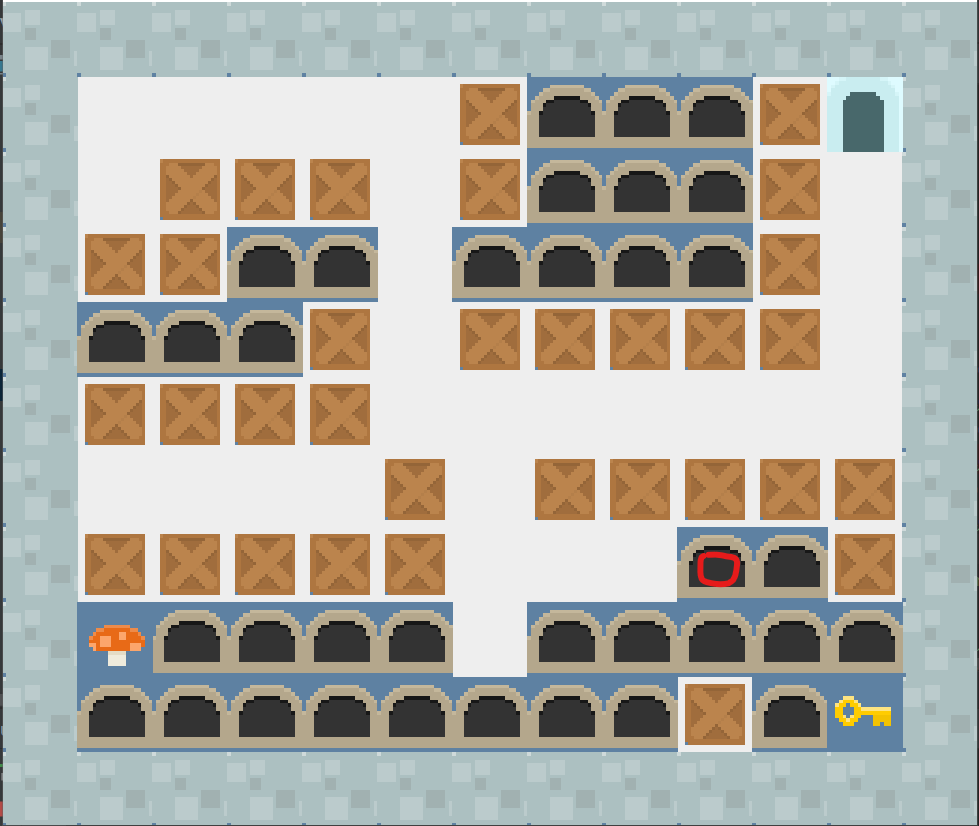
\includegraphics[width=10cm]{ai1-3.png}
	\caption{上述A*实现应用于第三关}
\end{figure}

\indent\textbf{原因分析}:\\
\indent 由于agent需要在有限的时间内决定一次行动,根据之前设计的预测函数,agent往往会向离goal较近的方向移动,而观察第二、三关结构发现,这两关都需要运用一定的策略填补坑洞,即先前往离目标较远的地方,这是已经设计的预测函数无法进行引导的。\\

\indent\textbf{改进}\\
\indent 1、考虑在对状态预测时,将填上的洞的数目作为一个衡量标准,从而鼓励agent多填洞,尤其可以对靠近目标(门、钥匙、蘑菇)的洞赋予更低的权值。\\
\indent 2、与1类似,也可以对箱子赋权,当箱子靠近墙或其他箱子时权值较高,而周围没有无法移动物体时权值较高。\\
\indent 3、关于蘑菇的处理:由于蘑菇并不是一定需要的,因此不适合将蘑菇作为goal,而是将目标和蘑菇之间的距离作为状态预测的又一个衡量标准,从而鼓励其前往蘑菇(但钥匙依旧具有绝对优先级)。\\

\section{MCTS介绍}
\noindent MCTS算法主要由以下三步组成:\\
\indent\textbf{1、随机漫步:}\\
\indent 对于每一次决策,将随机漫步的起点初始化为当前状态(调用init),之后不断重复以下动作直到到达规定时间:\\
\indent a、选择一个状态(tree\_policy): 如果当前状态存在未访问次态,那么随机选择其中一个未访问次态(tree\_expand),否则则最所有次态的置信度通过UCB公式进行评估,贪心地将最大置信度的次态更新为当前状态(uct),并再重复之前过程。\\
\indent b、从1中选择的状态开始,随机地选择行动,直到游戏结束或到达最大设定深度(此处设置为10),则停止行动(rollOut),并对终止状态进行评估,并维护评估结果的范围。\\
\indent\textbf{2、对状态进行评估并记录:}\\
\indent 评估方法(value):如果玩家胜利则估值为一个预先设定的较大数,失败为设立的一较小数,否则则为当前状态的分数。\\
\indent 记录(backUp):在之后不断回溯,并将具体的评估信息记录在其所有祖先结点中,增加祖先结点的访问次数以及总评估值。\\
\indent\textbf{3、返回评估最优的行为}(mostVistedAction):\\
\indent 到达设定的时间后,返回当前最优的行动,判定方法为:优先考虑访问次数最多的次态对应的行为,若所有次态访问次数均相等,则返回UCB公式下平均权值最大的次态对应的行为。\\
\noindent 总而言之,MCTS算法主要是随机搜索路径,对路径进行评估,记录信息并优化随机策略,继续随机搜索,最后返回搜索到的最优解的过程。\\


\end{document}


	
	
